\section{Generative Adversarial Networks~--~GANs}\label{GAN}

``When a deep neural network is used to generate data, the corresponding density function may be computationally intractable'' \citep{goodfellowGAN}. Unlike traditional generative models, implicit generative models do not require the explicit design of a density function to describe the patterns in the data. Instead, they use a sample generation process that produces new samples resembling the existing ones \citep{goodfellowGAN}. Before Generative Adversarial Networks were introduced, the leading implicit generative model was the generative stochastic network, ``which is capable of approximately generating samples via an incremental process based on Markov chains'' \citep{goodfellowGAN}. Markov chains are a way of describing a sequence of events or states, where probability of transition to the succeeding state is solely dependent on current states. This approach, however, can be time-intensive and may not always yield accurate results. GANs, on the other hand, directly generate high-quality samples in a single step, bypassing the gradual and often inefficient process of incremental generation.

The unique adversarial nature of GANs arises from the game-like competition between two neural networks: the generator and the discriminator. The generator is responsible for creating fake inputs or samples, which are then passed to the discriminator. The discriminator's role is to differentiate between real samples from the domain set and the fake samples generated by the generator.

\begin{figure}[ht]
\centering
  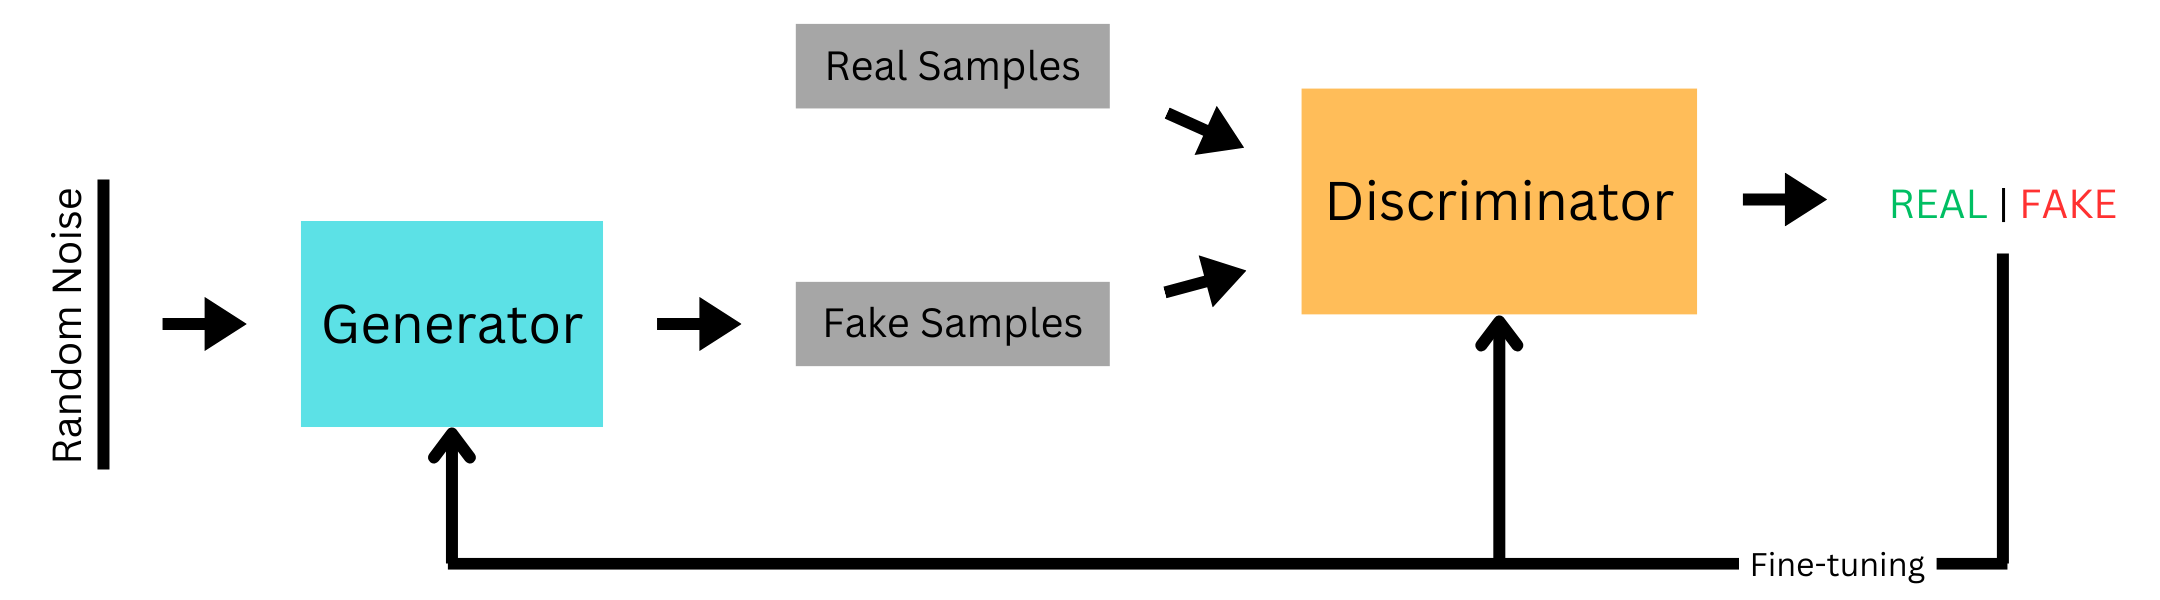
\includegraphics[width=1\columnwidth]{figures/Generator.png}
  \caption{Schematic representation of Generative Adversarial Networks showcasing the interaction between the generator and discriminator networks in generating new data.}\label{fig:figureGAN}
\end{figure}

In the initial training phase, the discriminator is trained on a dataset of real, unlabeled data, learning to identify the characteristics of authentic samples. As the discriminator becomes adept at recognizing all details, the generator starts creating counterfeits, using random input vectors to produce imitations. The discriminator then evaluates these fakes and provides feedback. This feedback loop, involving sample creation and model adjustments, gradually refines the generator's output. Eventually, the generator becomes so proficient that its fakes are indistinguishable from real data, achieving what is known as a zero-sum game, where one network's gain is the other's loss \citep{goodfellowGAN}.

However, the utility of GANs extends far beyond just image generation. Their applications encompass a wide range of fields, demonstrating their versatility and significant impact. These applications include video frame prediction, which is essential in multimedia applications; image enhancement, crucial in improving the quality and clarity of visual data; and encryption, where GANs contribute to the development of advanced security protocols \citep{goodfellowGAN}. One of the most notable features of GANs is their ability to learn in an unsupervised manner, particularly through the generator network. Unlike traditional models that require a supervised learning set with labeled data, GANs can generate new data after training the discriminator with real examples. This capability allows GANs to produce realistic and varied outputs without direct exposure to or reliance on a large labeled dataset \citep{GoodfellowDeepLearning},

% Additionally, GANs play a pivotal role in 3D object generation, the medical field,computer vision as well as traffic control systems, aiding in the development of smarter and more efficient transportation management \citep{AGGARWAL2021100004}.

Nevertheless, GANs pose a substantial challenge in their training process as they are hard to train \citep{goodfellowGAN}. In addition, \citeauthor{brophyGAN} highlight three important problems commonly associated with GANs, among others. These issues, namely non-convergence, diminishing or vanishing gradients, and mode collapse, contribute to the inherent instability experienced during GAN training. Non-convergence refers to the failure of a GAN model to stabilize and reach a state of equilibrium. Instead, it continuously oscillates and fails to converge to a satisfactory solution. As a result, the model does not learn the underlying patterns of the data and can even diverge, leading to poor performance \citep{brophyGAN}. Diminishing or vanishing gradients occur when the gradients used to update the generator become extremely small or even vanish altogether. This phenomenon is often caused by an overly successful discriminator that becomes too adept at distinguishing real and fake samples. As a result, the generator struggles to learn from the feedback provided by the discriminator, impeding its ability to generate high-quality samples \citep{brophyGAN}. Mode collapse happens when the generator collapses, meaning it focuses on producing only a limited set of samples or outputs, typically lacking diversity and variety \citep{salimansNIPS}. In such cases, the generator fails to capture the full range of patterns and characteristics present in the training data, resulting in uniform and repetitive samples that do not adequately represent the true distribution \citep{brophyGAN}.